
\subsubsection{5.1 Primary Finding: Corpus-Quality Hypothesis Refuted}

The corpus-quality $\rightarrow$ generalization-balance prediction is directly refuted. Pythia-6.9B achieves a higher MMLU/HellaSwag ratio than OLMo-7B at matched training scale, opposite to the hypothesis direction.

\textbf{Table 3: Benchmark Results at Approximately 300 Billion Training Tokens}

\begin{table*}[htbp]
\centering
\resizebox{\dimexpr 2\columnwidth+\columnsep\relax}{!}{%
\begin{tabular}{llllll}
\toprule
Model & Corpus & MMLU 5-shot & HellaSwag 0-shot & ARC-Easy 25-shot & ARC-Challenge 25-shot \\
\midrule
Pythia-6.9B & The Pile (minimal curation) & **0.2588** & **0.4580** & **0.6700** & **0.3360** \\
OLMo-7B & Dolma (multi-stage curation) & 0.2463 & 0.4580 & 0.6400 & 0.2960 \\
\bottomrule
\end{tabular}
}
\end{table*}

Pythia-6.9B achieves higher or equal performance on all four individual benchmarks. The MMLU gap is 0.0125 in favor of Pythia (0.2588 vs. 0.2463). HellaSwag scores are identical at 0.4580 for both models. ARC-Easy and ARC-Challenge both favor Pythia (0.0300 and 0.0400 absolute differences, respectively). The consistent directional pattern across all metrics makes the refutation robust to choice of aggregation method.

\subsubsection{5.2 Primary Metric: MMLU/HellaSwag Generalization Balance Ratio}

\begin{figure}[htbp]
\centering
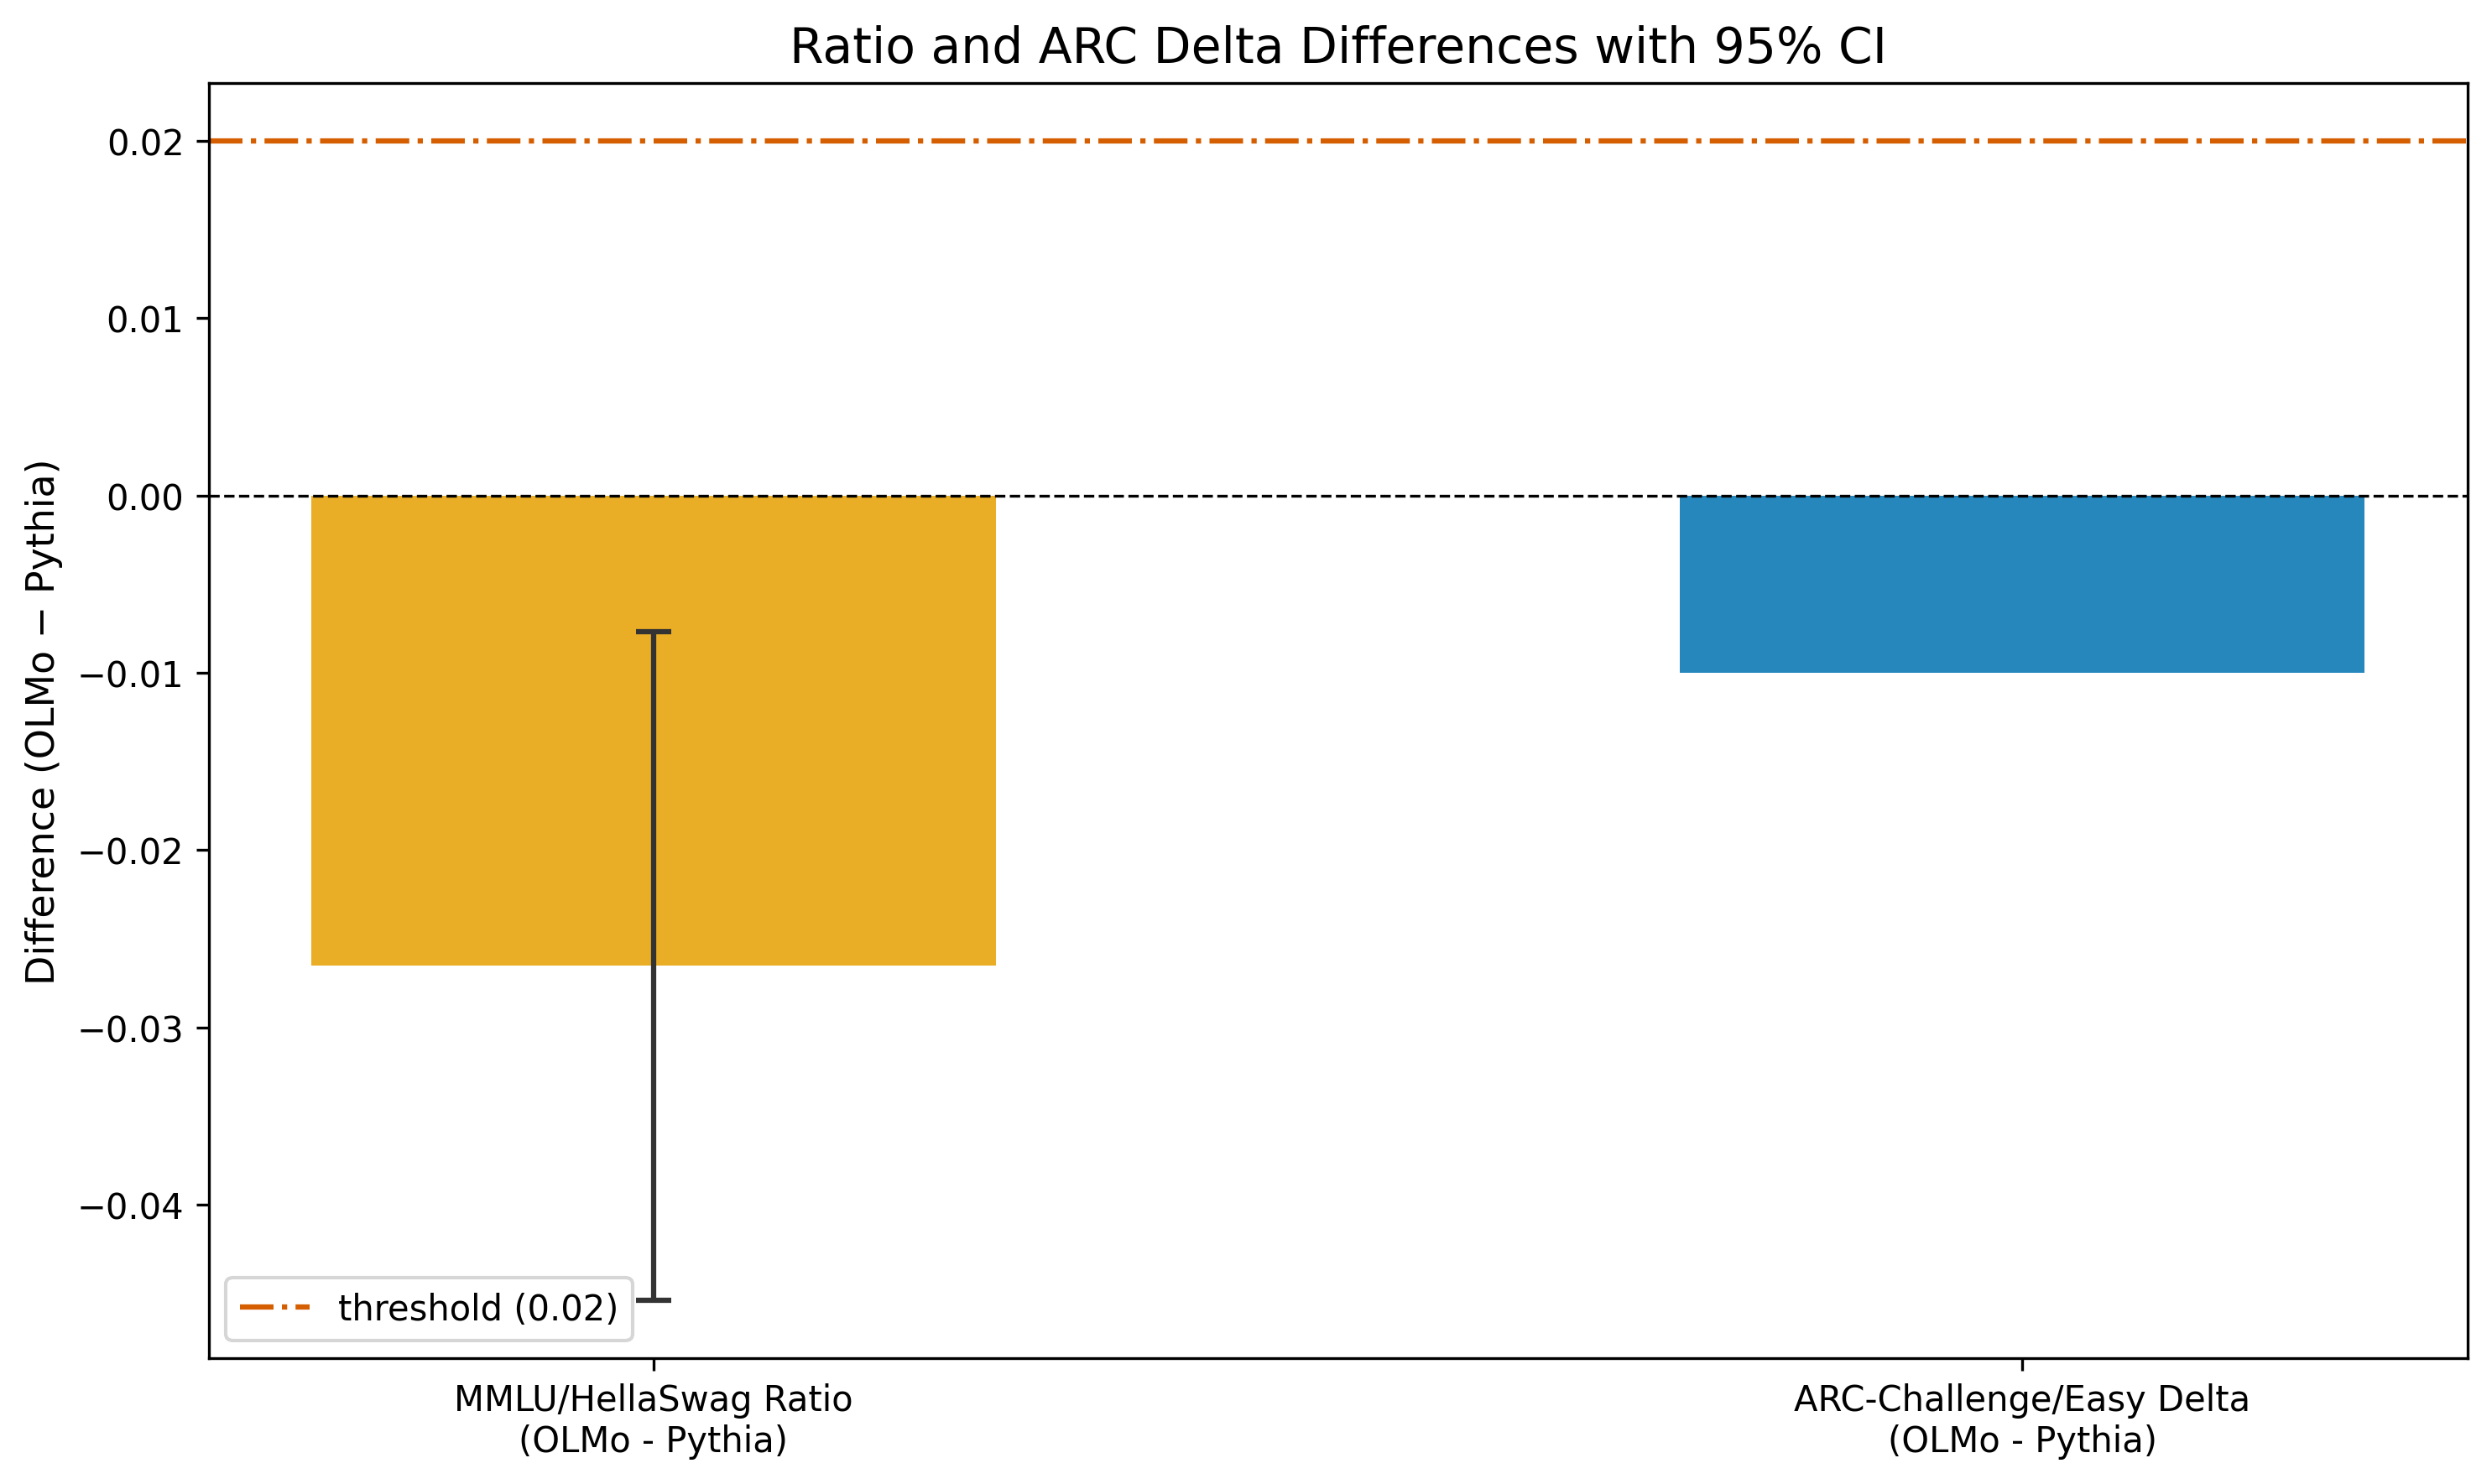
\includegraphics[width=\columnwidth]{figures/ratio_delta.png}
\caption{MMLU/HellaSwag ratio comparison with 95\% bootstrap CI}
\label{fig:ratio_delta}
\end{figure}

\textit{Figure 1: MMLU/HellaSwag generalization balance ratio for Pythia-6.9B and OLMo-7B with 95\% bootstrap confidence intervals. The hypothesis predicted OLMo $-$ Pythia > +0.02; the observed difference is $-0.0267$.}

\textbf{Table 4: Primary Metric Summary}

\begin{table*}[htbp]
\centering
\resizebox{\dimexpr 2\columnwidth+\columnsep\relax}{!}{%
\begin{tabular}{llllll}
\toprule
Metric & Pythia-6.9B & OLMo-7B & Difference (OLMo $-$ Pythia) & 95\% CI & Cohen's d \\
\midrule
MMLU/HellaSwag ratio & 0.5650 & 0.5383 & $-0.0267$ & [$-0.0447, -0.0069]$ & $-2.732$ \\
ARC delta (Challenge $-$ Easy) & $-0.3340$ & $-0.3440$ & $-0.0100$ (OLMo worse) & --- & --- \\
\bottomrule
\end{tabular}
}
\end{table*}

The hypothesis predicted OLMo $-$ Pythia > +0.02; the observed value is $-0.0267$. The bootstrap 95\% CI on the ratio difference lies entirely below zero. The one-sided p-value for the test that OLMo $\geq$ Pythia is 0.996, indicating that only 0.4\% of bootstrap iterations produced an OLMo ratio exceeding Pythia's. Cohen's d = $-2.732$ indicates a large effect in the direction opposite to the prediction. All three pre-registered gate criteria (ratio difference > 0.02, Cohen's d > 0.2, one-sided p < 0.05) failed. The result is not a null result in the sense of no detectable effect; it is a large, statistically robust result in the direction opposite to the hypothesis.

\subsubsection{5.3 Secondary Metric: ARC-Challenge/Easy Delta}

Pythia-6.9B achieves an ARC-Challenge score of 0.3360 and ARC-Easy score of 0.6700, yielding a delta of $-0.3340$. OLMo-7B achieves 0.2960 and 0.6400, yielding a delta of $-0.3440$. OLMo's delta is more negative by 0.0100, indicating greater degradation from easy to challenge-level reasoning. The directional refutation is confirmed across both primary and secondary metrics.

\subsubsection{5.4 Analysis: HellaSwag Convergence as a Structural Finding}

\begin{figure}[htbp]
\centering
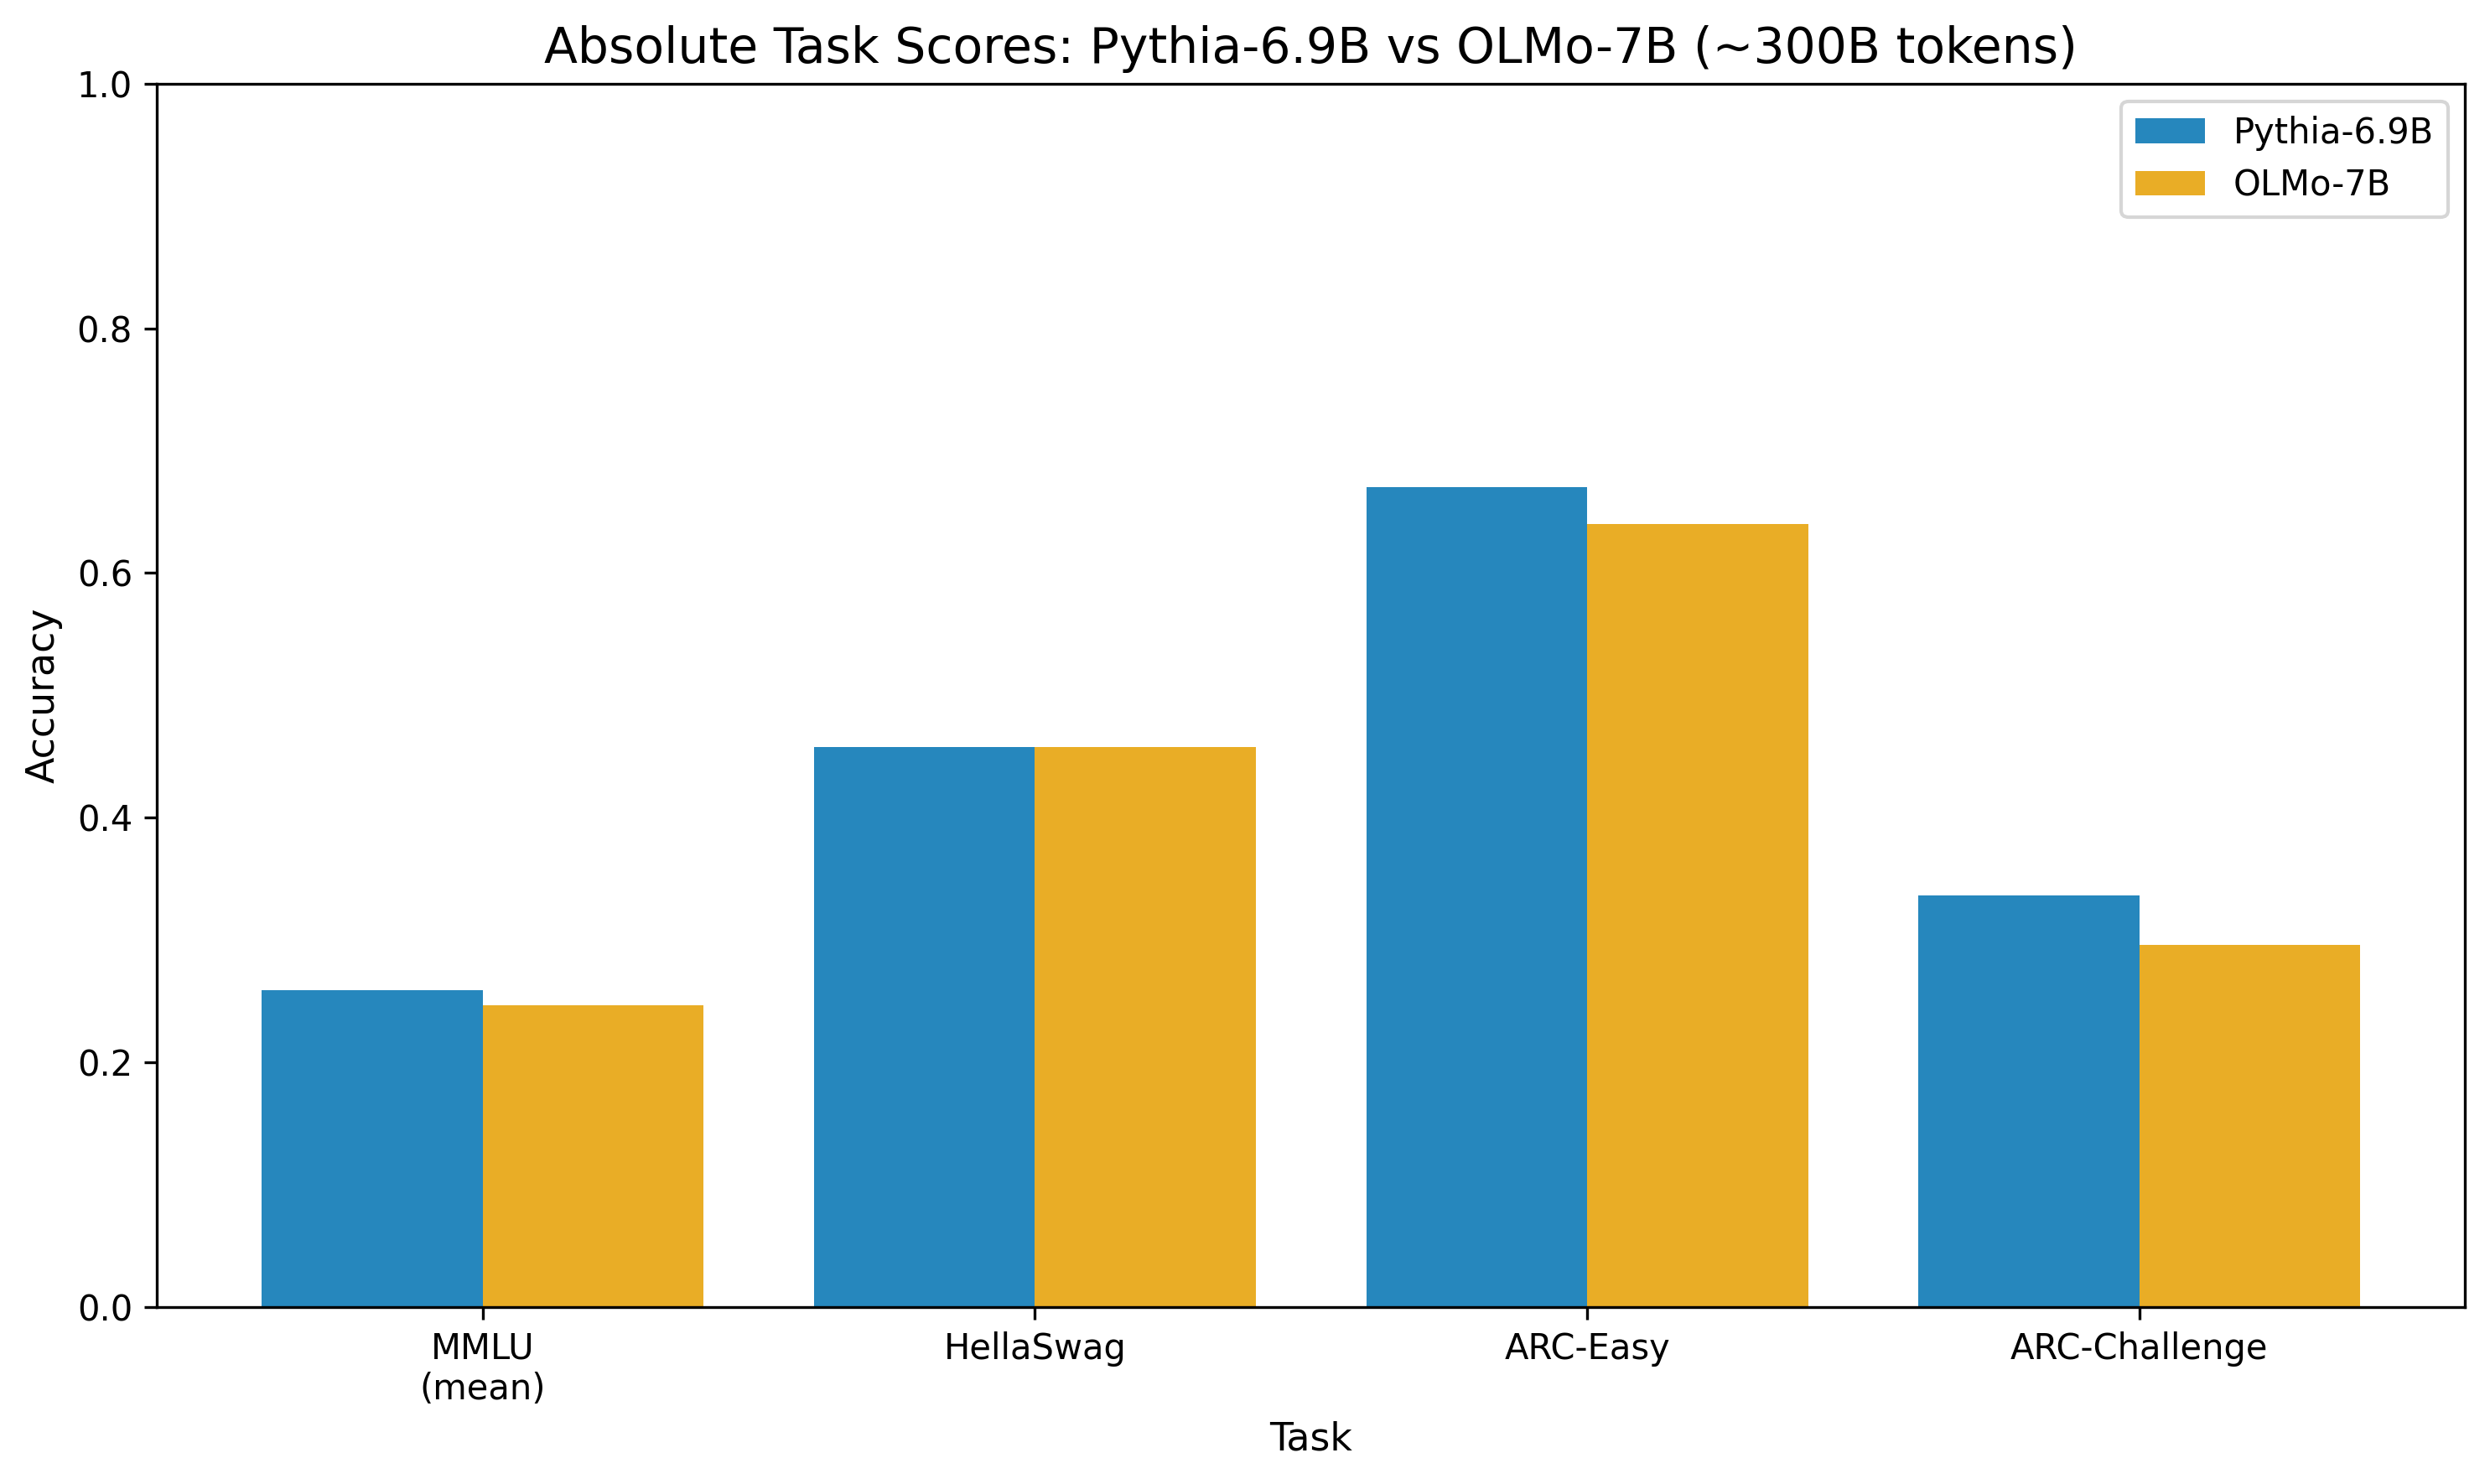
\includegraphics[width=\columnwidth]{figures/absolute_scores.png}
\caption{All four benchmark scores for Pythia-6.9B and OLMo-7B}
\label{fig:absolute_scores}
\end{figure}

\textit{Figure 2: Side-by-side comparison of all four benchmark scores for both models at approximately 300 billion training tokens.}

The identical HellaSwag scores (0.4580 for both models in fast evaluation) are structurally significant. Three explanations are considered:

\begin{enumerate}
\item \textbf{Scale-dependent saturation (HIGH plausibility).} At approximately 300 billion tokens, 6--8 billion parameter models have absorbed sufficient web-sourced commonsense content --- present in both The Pile and Dolma via CommonCrawl --- to reach a convergent performance ceiling on HellaSwag. This is consistent with Biderman et al. [2023], who show that deduplication gains on HellaSwag are approximately 0.01 absolute within the Pythia suite, suggesting limited discriminative power of the task for corpus quality differences in this model family.
\end{enumerate}

\begin{enumerate}
\item \textbf{Sampling variance (MEDIUM plausibility).} With approximately 500 evaluation examples, identical scores to three decimal places could arise by chance. Full evaluation with the complete 10,042-example HellaSwag validation set is needed to confirm.
\end{enumerate}

\begin{enumerate}
\item \textbf{Task insensitivity to quality differences (MEDIUM plausibility).} HellaSwag's commonsense content is well-represented in both corpora via CommonCrawl, making it inherently insensitive to quality differences between The Pile and Dolma at this scale.
\end{enumerate}

The key structural implication is: when the denominator of the MMLU/HellaSwag ratio is a constant (0.4580), the ratio reduces algebraically to MMLU / 0.4580. The observed ratio difference of $-0.0267$ is entirely driven by the MMLU gap of 0.0125. HellaSwag provides no discriminative information in this comparison, and the MMLU differences are confounded by the architecture difference between the two models.

\subsubsection{5.5 Per-Subject MMLU Heatmap and Contamination Assessment}

\begin{figure}[htbp]
\centering
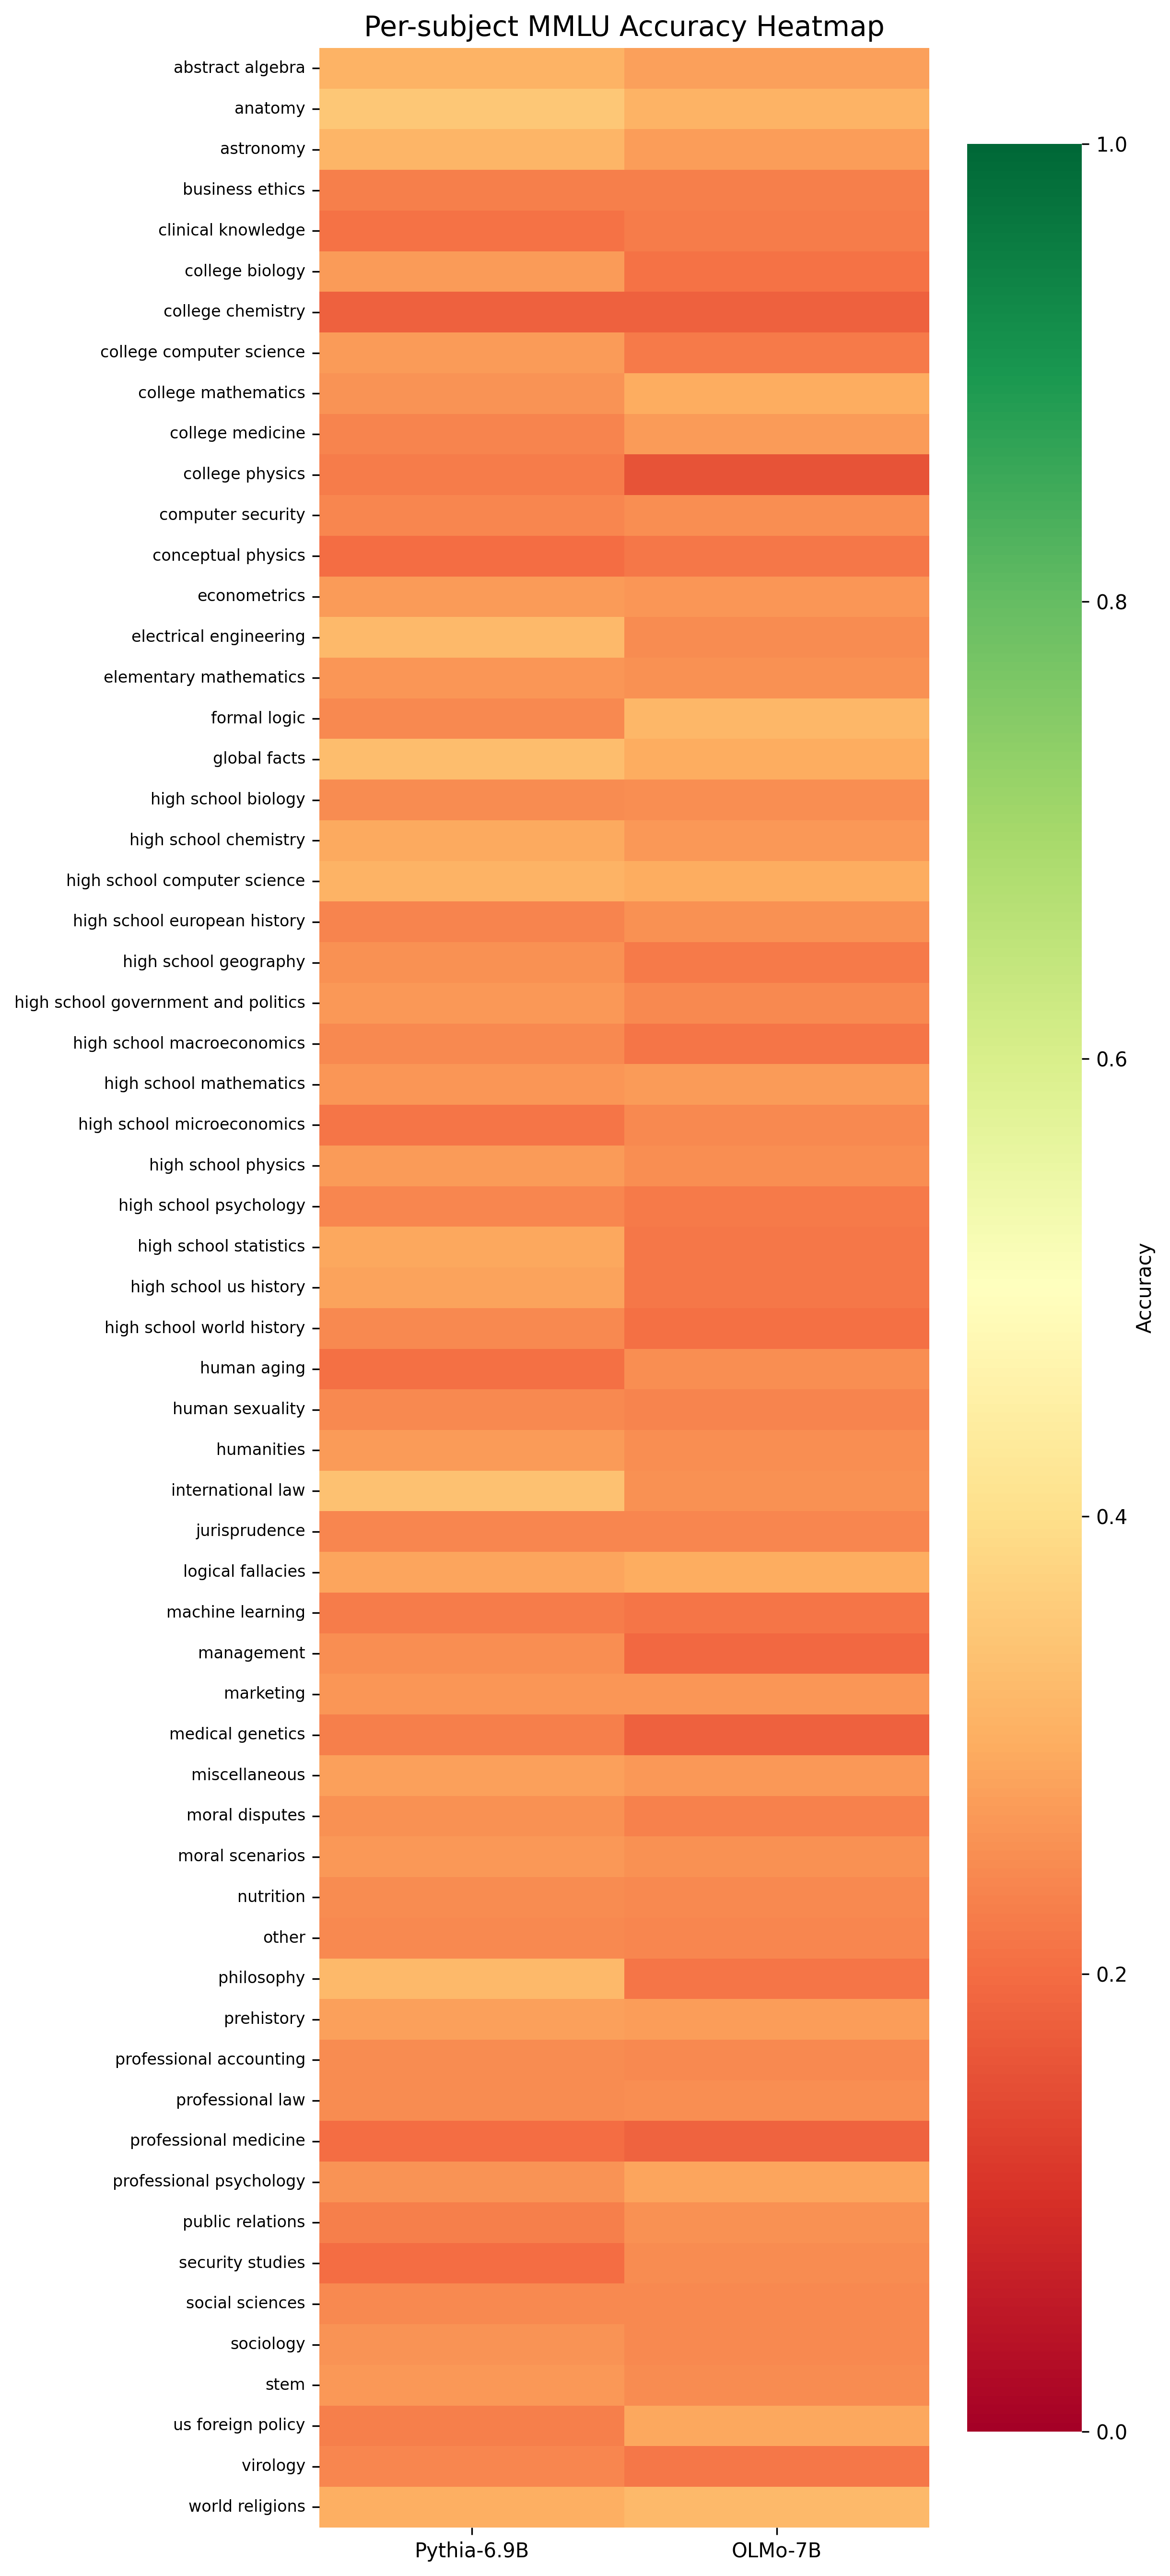
\includegraphics[width=\columnwidth]{figures/mmlu_heatmap.png}
\caption{Per-subject MMLU accuracy heatmap for all 57 subjects}
\label{fig:mmlu_heatmap}
\end{figure}

\textit{Figure 3: Per-subject MMLU accuracy for Pythia-6.9B and OLMo-7B across 57 MMLU subjects. Pythia's advantage is broadly distributed rather than concentrated in specific domains.}

The per-subject heatmap shows Pythia's MMLU advantage is broadly distributed across subjects including STEM (physics, chemistry, biology), social sciences (economics, law, psychology), and humanities (history, philosophy). This pattern is inconsistent with The Pile contamination as the primary explanation: contamination would be expected to concentrate in domains well-represented in The Pile's specific sources (e.g., PubMed for medicine, ArXiv for physics, legal databases for law). The absence of domain concentration reduces the plausibility of contamination, though it does not rule it out. Min-K\% contamination detection \citep{Shi2024MinK} applied to MMLU test questions against The Pile would provide more definitive evidence.

\subsubsection{5.6 Bootstrap Distribution}

\begin{figure}[htbp]
\centering
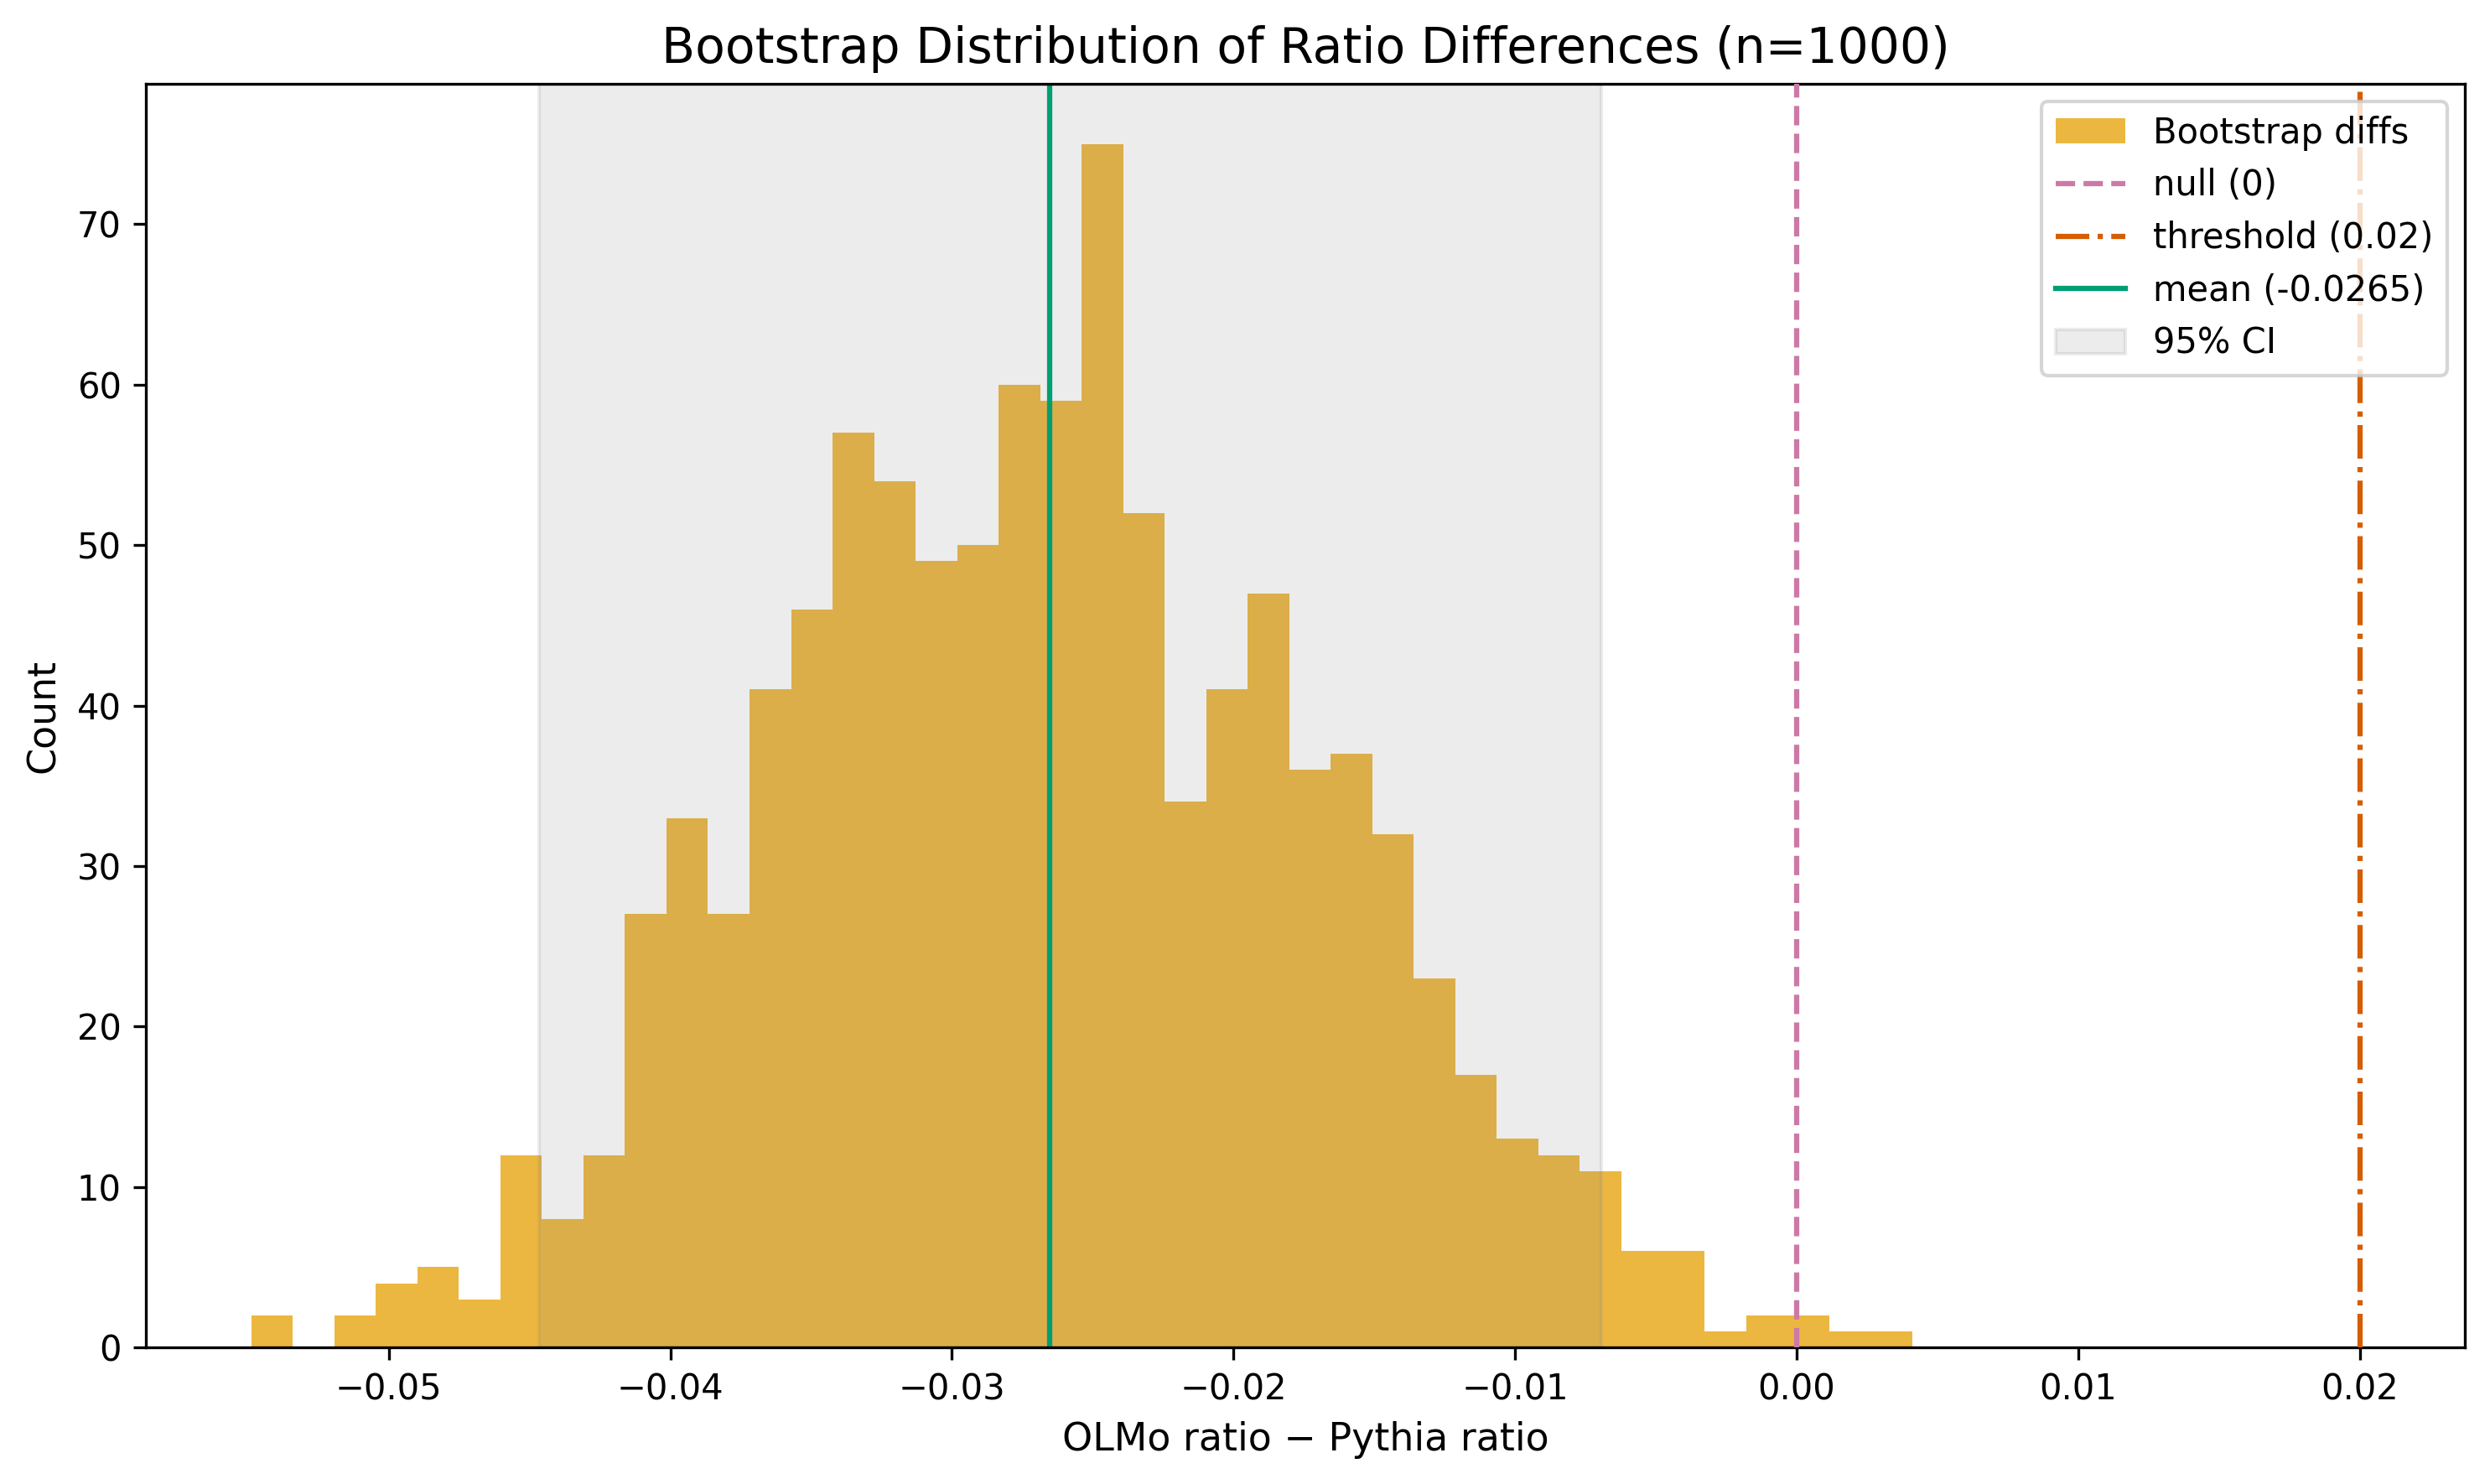
\includegraphics[width=\columnwidth]{figures/bootstrap_dist.png}
\caption{Bootstrap distribution of ratio differences}
\label{fig:bootstrap_dist}
\end{figure}

\textit{Figure 4: Bootstrap distribution of ratio differences (OLMo $-$ Pythia) across 1,000 iterations. Dashed vertical line at 0 (null hypothesis); dotted vertical line at +0.02 (hypothesis threshold). Neither falls within the distribution.}

The bootstrap distribution is centered at $-0.0265$ and lies entirely below zero. Neither the null value (0) nor the hypothesis threshold (+0.02) falls within the distribution. The 95\% CI of [$-0.0447, -0.0069]$ excludes zero, confirming that the directional refutation is statistically robust to MMLU subject-level sampling variance.

\subsubsection{5.7 Summary of Research Questions}

\textbf{RQ1:} Pythia-6.9B achieves a significantly higher MMLU/HellaSwag ratio than OLMo-7B (0.5650 vs. 0.5383, d = $-2.732$, 95\% CI entirely negative). The hypothesis is directly falsified.

\textbf{RQ2:} OLMo-7B does not achieve a less-negative ARC delta. Pythia's delta ($-0.334)$ is less negative than OLMo's ($-0.344)$, confirming the directional refutation via an independent metric.

\textbf{RQ3:} Pythia's MMLU advantage is broadly distributed across subjects, inconsistent with domain-specific contamination from The Pile as the primary explanation.

